\documentclass[12pt]{article}
%% arXiv paper template by Flip Tanedo
%% last updated: Dec 2016



%%%%%%%%%%%%%%%%%%%%%%%%%%%%%
%%%  THE USUAL PACKAGES  %%%%
%%%%%%%%%%%%%%%%%%%%%%%%%%%%%

\usepackage{amsmath}
\usepackage{amssymb}
\usepackage{amsfonts}
\usepackage{graphicx}
\usepackage{xcolor}
\usepackage{nopageno}
\usepackage{enumerate}
\usepackage{parskip}

%%%%%%%%%%%%%%%%%%%%%%%%%%%%%%%%%
%%%  UNUSUAL PACKAGES        %%%%
%%%  Uncomment as necessary. %%%%
%%%%%%%%%%%%%%%%%%%%%%%%%%%%%%%%%

\usepackage{tikzfeynman}

\usepackage{titlesec}
\titleformat*{\section}{\large\bfseries}

%% MATH AND PHYSICS SYMBOLS
%% ------------------------
%\usepackage{slashed}       % \slashed{k}
%\usepackage{mathrsfs}      % Weinberg-esque letters
%\usepackage{youngtab}	    % Young Tableaux
%\usepackage{pifont}        % check marks
\usepackage{bbm}           % \mathbbm{1} incomp. w/ XeLaTeX 
%\usepackage[normalem]{ulem} % for \sout


%% CONTENT FORMAT AND DESIGN (below for general formatting)
%% --------------------------------------------------------
\usepackage{lipsum}        % block of text (formatting test)
%\usepackage{color}         % \color{...}, colored text
%\usepackage{framed}        % boxed remarks
%\usepackage{subcaption}    % subfigures; subfig depreciated
%\usepackage{paralist}      % compactitem
%\usepackage{appendix}      % subappendices
%\usepackage{cite}          % group cites (conflict: collref)
%\usepackage{tocloft}       % Table of Contents	

%% TABLES IN LaTeX
%% ---------------
%\usepackage{booktabs}      % professional tables
%\usepackage{nicefrac}      % fractions in tables,
%\usepackage{multirow}      % multirow elements in a table
%\usepackage{arydshln} 	    % dashed lines in arrays

%% Other Packages and Notes
%% ------------------------
%\usepackage[font=small]{caption} % caption font is small



%\renewcommand{\thesection}{}
%\renewcommand{\thesubsection}{\arabic{subsection}}

%%%%%%%%%%%%%%%%%%%%%%%%%%%%%%%%%%%%%%%%%%%%%%%
%%%  PAGE FORMATTING and (RE)NEW COMMANDS  %%%%
%%%%%%%%%%%%%%%%%%%%%%%%%%%%%%%%%%%%%%%%%%%%%%%

\usepackage[margin=2cm]{geometry}   % reasonable margins

\graphicspath{{figures/}}	        % set directory for figures

% for capitalized things
\newcommand{\acro}[1]{\textsc{\MakeLowercase{#1}}}    

\numberwithin{equation}{section}    % set equation numbering
\renewcommand{\tilde}{\widetilde}   % tilde over characters
\renewcommand{\vec}[1]{\mathbf{#1}} % vectors are boldface

\newcommand{\dbar}{d\mkern-6mu\mathchar'26}    % for d/2pi
\newcommand{\ket}[1]{\left|#1\right\rangle}    % <#1|
\newcommand{\bra}[1]{\left\langle#1\right|}    % |#1>
\newcommand{\Xmark}{\text{\sffamily X}}        % cross out

% Change list spacing (instead of package paralist)
% from: http://en.wikibooks.org/wiki/LaTeX/List_Structures#Line_spacing
%\let\oldenumerate\enumerate
%\renewcommand{\enumerate}{
%  \oldenumerate
%  \setlength{\itemsep}{1pt}
%  \setlength{\parskip}{0pt}
%  \setlength{\parsep}{0pt}
%}

\let\olditemize\itemize
\renewcommand{\itemize}{
  \olditemize
  \setlength{\itemsep}{1pt}
  \setlength{\parskip}{0pt}
  \setlength{\parsep}{0pt}
}


% Commands for temporary comments
\newcommand{\comment}[2]{\textcolor{red}{[\textbf{#1} #2]}}
\newcommand{\flip}[1]{{\color{red} [\textbf{Flip}: {#1}]}}
\newcommand{\email}[1]{\texttt{\href{mailto:#1}{#1}}}

\newenvironment{institutions}[1][2em]{\begin{list}{}{\setlength\leftmargin{#1}\setlength\rightmargin{#1}}\item[]}{\end{list}}


\usepackage{fancyhdr}		% to put preprint number



% Commands for listings package
\usepackage{listings}      % \begin{lstlisting}, for code
%
 \lstset{basicstyle=\ttfamily\footnotesize,breaklines=true}
%    sets style to small true-type


%%%%%%%%%%%%%%%%%%%%%%%%%%%%%%%%%%%%%%%%%%%%%%
%%%  TIKZ COMMANDS FOR EXTERNAL DIAGRAMS  %%%%
%%%  requires -shell-escape               %%%%
%%%  in texpad 1.7: prefs > shell esc sec %%%%
%%%%%%%%%%%%%%%%%%%%%%%%%%%%%%%%%%%%%%%%%%%%%%

%% This is for exporting tikz figures as into a ./tikz/ subfolder.
%% It is useful if you want pdf versions of the tikz diagrams or
%% if you need to speed up compilation of a large document with
%% many tikz diagrams.

%\write18{} % Careful with this!
%\usetikzlibrary{external}
%\tikzexternalize[prefix=tikz/] % folder for external pdfs


%%%%%%%%%%%%%%%%%%%
%%%  HYPERREF  %%%%
%%%%%%%%%%%%%%%%%%%

%% This package has to be at the end; can lead to conflicts
\usepackage{microtype}
\usepackage[
	colorlinks=true,
	citecolor=black,
	linkcolor=black,
	urlcolor=green!50!black,
	hypertexnames=false]{hyperref}



%%%%%%%%%%%%%%%%%%%%%
%%%  TITLE DATA  %%%%
%%%%%%%%%%%%%%%%%%%%%

%%% PREPRINT NUMBER USING fancyhdr
%%% Don't forget to set \thispagestyle{firststyle}
%%% ----------------------------------------------
%\renewcommand{\headrulewidth}{0pt} % no separator
%\fancypagestyle{firststyle}{
%\rhead{\footnotesize \texttt{UCI-TR-2016-XX}}}



\begin{document}

%\thispagestyle{empty}
%\thispagestyle{firststyle} %% to include preprint

\begin{center}

    {\Large \textsc{Homework 4:} 
    \textbf{Operators on Function Space}}


    
\end{center}

\vskip .4cm

\noindent
\begin{tabular*}{\textwidth}{rlcrll}
	\textsc{Course:}& Physics 231, \emph{Methods of Theoretical Physics} (2017)
	&
%	\hspace{1.2cm}
	&
	\\
	\textsc{Instructor:}& Flip Tanedo (\email{flip.tanedo@ucr.edu})
	&
	%\hfill
	&
	& 
	\\
	\textsc{Due by:}& Friday, October 27
	&
	%\hfill
	&
	%	
\end{tabular*}



\textbf{Reading}: For this week, please read your favorite references to brush up on complex analysis. Our main goal is to understand contour integrals, though we will take a detour and see a nice application to causality. Please review the following key topics: 
\begin{itemize}
\item The Cauchy--Riemann equations
\item The meaning of an analytic function
\item Laurent series
\item Cauchy's theorem
\item The residue theorem.	
\end{itemize}
 Some possible references include: Byron \& Fuller chapter 6, Boas chapter 14, Matthews \& Walker chapter 3.3 and appendix A, Stone \& Goldbart chapter 17, Appel chapter 4.1--4.6, Cahill chapter 5.1--5.14.


\section{Sturm--Liouville Operator}

% See Matthews & Walker 9-2
% Stone and Goldbart 4.2

This problem follows Lecture 9. Consider the differential operator
\begin{align}
	L = p_2(x) \left(\frac{d}{dx}\right)^2
	+ p_1(x)\frac{d}{dx}
	+ p_0(x) .
\end{align}
Assume $w(x) = 1$ and some domain $x\in [a,b]$.

\textsc{Reference}: Refer to Stone \& Goldbart chapter 4 for a discussion of formal versus concrete (what we called `proper') linear differential operators. We use a slightly different notation, but the question of a formal adjoint is explored in 4.2 with the Sturm--Liouville operator identified in equation (4.28). A more general discussion that follows more of the spirit of the lecture is in Matthews \& Walker Chapter 9-2.

\subsection{Formal adjoint}
Using integration by parts, show that the formal adjoint of this operator is 
\begin{align}
	L^\dag = \left(\frac{d}{dx}\right)^2 p_2(x)
	- \left(\frac{d}{dx}\right)p_1(x)
	+ p_0(x) \ ,
\end{align}
where we use the notation 
\begin{align}
	\left[\left(\frac{d}{dx}\right)^n p_n(x)\right] f(x) \equiv 
		\left(\frac{d}{dx}\right)^n 
		\left[ p_n(x)\, f(x)\right] \ .
\end{align}

\subsection{Self-Adjoint Case}

Show that in order for $L$ to be formally self-adjoint, that is $L = L^\dag$ (without considering boundary conditions), then the following conditions must hold:
\begin{align}
	p_1(x) &= 2p_2'(x) - p_1(x) \\
	p_0(x) &= p_x''(x) - p_1(x) + p_0(x) \ .
\end{align}
Thus $L$ is self-adjoint (Hermitian) if $p_1(x) = p_2'(x)$. $L$ can be written succinctly as:
\begin{align}
	L &= \frac{d}{dx}
		\left(p_2(x)\frac{d}{dx}\right) + p_0(x) \ .
\end{align}




\section{A Green's function by completeness}

% Matthews and Walker 9-4
% Stone & Goldbart 5.4
% Cahill 6.38
% Byron and Fuller 7.2

%\textcolor{blue}{\textbf{Correction} (10/27, after due date): The $(d/dx)^2$ operator is not self-adjoint. As we saw in class, the formally self adjoint operator is $-(d/dx)^2$. As a result, the eigenvalues of $(d/dx)^2$ are negative rather than positive. Thanks to Wei-Xiang Feng for catching this.}

Three formulaic ways of solving for Green's functions are:
\begin{enumerate}
	\item Fourier transforming to turn the differential operator into an algebraic one, and then doing a contour integral to go back to position space.
	\item Solving the homogeneous equation and patching together two solutions over the $\delta$-function. 
	\item Using the completeness of eigenfunctions.
\end{enumerate}
We will spend most of this course highlighting method 1. Next week you will use method 2---it will be familiar from electrodynamics. This week, we will use the third method, which is based on the eigenfunction completeness relation,
\begin{align}
	\sum_n e_n^*(y) e_n(x) = \delta(x-y) \ .
\end{align}
Thus if you know the eigenvalues of the linear differential operator, $L_x$, then you can use this relation to hack together the Green's function $G$ because $L_x G(x,y) = \delta(x-y)$.  The subscript $x$ in $L_x$ means that the operator is a function of $x$ and derivative operators with respect to $x$.

\textsc{References}: This method is discussed in  Matthews \& Walker chapter 9-4, Stone \& Goldbart chapter 5.4, Cahill chapter 6.38, and Byron \& Fuller chapter 7.2. 

In this problem, we consider a second order differential equation acting on a state $\psi(x)$ with a source $s(x)$. 
\begin{align*}
	\left(\frac{d^2}{dx^2} + k^2 \right) \psi(x) = s(x) \ .
\end{align*}
We consider the domain $x\in[0,1]$ with boundary conditions $\psi(0) = \psi(1) = 0$.

\subsection{Eigenfunctions}

What are the eigenfunctions $e_n(x)$ and the corresponding eigenvalues $\lambda_n$? Recall that an eigenfunction of a linear operator $L_x$ satisfies $L_x e_n(x) = \lambda_n e_n(x)$. 


\textsc{Hint:} The eigenfunctions of $d^2/dx^2$ are $\psi_n(x) = \sqrt{2} \sin (n\pi x)$ with eigenvalues $n^2 \pi^2$. What changes when the operator $L_x$ includes an additive constant?


\subsection{Completeness}


Write down the Green's function $G(x,y)$ using the completeness trick with respect to eigenfunctions $e_n$ with eigenvalues $\lambda_n$: 
\begin{align}
	G(x,y) = \sum_n \frac{e_n^*(y)e_n(x)}{\lambda_n} \ .
\end{align}

\textsc{Hint:} Once you did the previous part, this step takes about twenty seconds depending on how quickly you write.


\subsection{Hands on}

You have a free license for several types of scientific software 
through \acro{UCR} through MySoftware\footnote{\url{http://cnc.ucr.edu/mysoftware/}}. This problem requires some plotting. I suggest using \emph{Mathematica}\footnote{It sucks that this is not open source software. The closest open source alternative is \texttt{SciPy} with a \texttt{Jupyer} notebook. You can use this instead if you prefer.}. 

Plot the solution to the Green's function $G(x,y)$ for $y = 0.5$ and $k = 0.2$, summing from $n=1$ to $n=10$. Here's the general way to format it in \emph{Mathematica}:
\begin{center}
	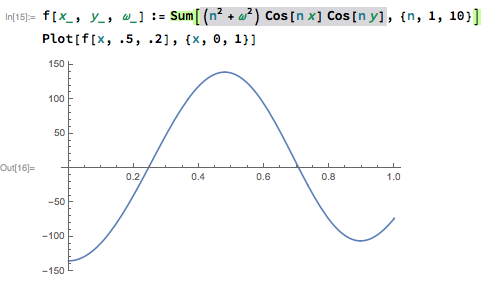
\includegraphics[width=.6\textwidth]{P231_2017_HW4_fig1.png}
\end{center}

The highlighted piece and the example plot are \emph{completely wrong}! Fill it in with the correct $G(x,y)$ and plot it. It may help to use the `Basic Math Input' palette if you're unfamiliar with this. If this task is very painful, please ask a friend. If this is still very painful, then you may use any other plotting program that you wish. 

Does this shape make sense? What do you expect will happen as $n$ becomes larger? Try it for $n=100$. Explore what happens as you change $k$ and $y$. (Make sure $y$ is in the domain of the function space!) Take a moment to have a nice warm cup of tea, enjoy the agreeable weather outside, and meditate upon why this shape of the Green's function makes sense and the kinds of physical problem where Green's function may be relevant. You do not have to write up these meditations, but I do strongly suggest the tea and outdoors\footnote{If you are looking for nice tea to bring home, I suggest the \emph{British Emporium} in Canyon Crest.}.  





\appendix
\section*{\Large Extra Credit}


These problems are not graded and are for your edification. You are strongly encouraged to explore and discuss these topics, especially if they are in a field of interest to you.

\section{Dimensional Analysis: Nature is Approximately Second Order} 

Most differential equations in physics are second order (in derivatives) or less. We observed that this can be understood from the mantra that \emph{physics is local}; higher derivative terms encode non-locality. Here we give a toy example for why nature appears to stop at second order.

Often our favorite differential equations come from a least action principle, $\delta S = 0$. In natural units, the action is dimensionless, $[S]=0$. We'll take the example of the dynamics of a scalar field, $h(x)$. This is a function defined over all of space and time. Quantum excitations of this field correspond to particles.

\begin{enumerate}[(a)]
	\item The action is written as an integral of a Lagrangian density, $\mathcal L$ over spacetime: $S = \int d^4x \, \mathcal L$. To match onto something familiar, this is just saying that $S = \int dt \, L$ with $L = \int d^3\mathbf{x} \, \mathcal L$. In natural units, what is the mass dimension of $\mathcal L$?
	\item The Lagrangian density is a function of the field $h(x)$ and derivatives, $\partial_\mu = \partial/\partial x^\mu$. A dynamical particle necessarily has at least the following term in the Lagrangian density, $$\mathcal L \supset \frac 12 h(x) \partial_\mu \partial^\mu h(x) = \frac 12 h(x) \left(\partial_t^2 - \partial_x^2 - \partial_y^2 - \partial_z^2\right) h(x).$$ This corresponds to the kinetic energy term in the Lagrangian. In natural units, what is the mass dimension of a derivative, $\partial_\mu$? (Does it matter whether it's a time derivative or a space derivative?) What is the mass dimension of the field $h(x)$?  Observe that Lorentz invariance requires that the space derivatives come along with the time derivatives.
	\item We can ignore terms in the Lagrangian density with fewer than two powers\footnote{Extra credit: think about such terms would mean for the differential equation that comes from $\delta S = 0$.} of $h(x)$. Lorentz invariance says that you cannot have a term with an odd number of derivatives, so let's imagine what would happen to a term in $\mathcal L$ that had two powers of $h(x)$ and four derivatives, for example: $$\mathcal L \supset \Lambda^n h(x) \partial^4 h(x) .$$ We've included an overall prefactor, $\Lambda^n$. Assume that $\Lambda$ has mass dimension of one. Given your answers to the previous question, what is the value of $n$ for which the $\mathcal O(\partial^4)$ term has the correct dimension for a Lagrangian density term?
	\item The answer to the above question is $n=-2$. One of the key ideas in theoretical physics is the \textit{renormalization group} (related ideas: effective theories, anomalous scaling.). I hope you have the chance to study this in the many ways it shows up in different fields, but one of the punchlines of this idea is that the prefactor $\Lambda^n$ in operators like the one above should be identified with a \emph{cutoff} for the theory. That is: this is an energy scale (inverse length scale) at which the model you're using to describe the system breaks down because you're not including micro-physics. For example: if you had an action for the behavior of water waves where the water is treated as a continuous medium, then the theory breaks down at the scale where individual water molecules are resolved. Is $\Lambda$ a `big' number or a `small' number? Specify in what sense you mean this---what units are you using, and to what are you comparing? \textsc{Hint}: As you know from Fourier analysis, derivatives bring down powers of momentum. So a more concrete question is: I have a theory of the scalar field $h(x)$ which I know is valid at some energy scale, $E$---if all my momenta are of this characteristic energy scale, $\partial \to k \approx E$, then is the coefficient of the $\mathcal O(\partial^4)$ term in (c) bigger or smaller than the ordinary kinetic term in (b)?
\end{enumerate}


\section{Self-adjointness and Variational Principles}

Kuntal brought up a great point on Wednesday: there is a relation between the self-adjointness of a differential operator appearing in an equation of motion whether or not that equation could come from a variational principle. There is some discussion online\footnote{\url{https://physics.stackexchange.com/q/291697}}, but I've yet to find a satisfactory physically intuitive explanation (to the extent to which the statement is even true). However, I suspect such an explanation relates reversibility and conservation of probability in quantum mechanics. If you have thoughts on this, I would be happy to hear them.


\end{document}